\documentclass[a4paper]{article}
\usepackage[14pt]{extsizes} % для того чтобы задать нестандартный 14-ый размер шрифта
\usepackage{amsmath}
\usepackage[unicode, pdftex]{hyperref} % гиперссылки
\usepackage[usenames]{color} %цвета
\usepackage{mathtext}
\usepackage[T2A]{fontenc}
\usepackage[utf8]{inputenc}
\usepackage[english, russian]{babel}
\usepackage{amsfonts}
\usepackage{float} % для нормального расположения картинок и таблиц
\usepackage[left=20mm, top=15mm, right=15mm, bottom=15mm, nohead, footskip=10mm]{geometry} % настройки полей документа
\usepackage{graphicx} % работа с картинками 
\usepackage{wrapfig}
\usepackage{placeins} % работа с картинками (их корректная вставка в текст)
\usepackage{misccorr} % в заголовках появляется точка, но при ссылке на них ее нет
\usepackage{indentfirst} % красная строка у первой строки раздела
\DeclareMathSymbol{,}{\mathord}{letters}{"3B} % убирает пробел после запятой в формулах
%% Определяем свой шрифт "lsumb"
\DeclareSymbolFont{lsymb}{U}{euex}{m}{n}
%% Определяем интегралы
\DeclareMathSymbol{\intop}{\mathop}{lsymb}{"52}
\DeclareMathSymbol{\ointop}{\mathop}{lsymb}{"48}
\DeclareMathSymbol{\smallint}{\mathop}{lsymb}{"52}
%Красивая ЭДС с завитушками
\usepackage{mathrsfs}
\DeclareSymbolFont{rsfs}{U}{rsfs}{m}{n} \DeclareSymbolFontAlphabet{\mathscr}{rsfs}
\DeclareMathSymbol{\EDS}{\mathord}{rsfs}{`E}
\usepackage{amssymb} %русские неравенства: \leqslant \geqslant

\begin{document}
\begin{center}
	\hfill \break
	{\small МИНИСТЕРСТВО НАУКИ И ВЫСШЕГО ОБРАЗОВАНИЯ РОССИЙСКОЙ ФЕДЕРАЦИИ}\\
	\hfill \break
	{\small ФЕДЕРАЛЬНОЕ ГОСУДАРСТВЕННОЕ АВТОНОМНОЕ ОБРАЗОВАТЕЛЬНОЕ\\ УЧРЕЖДЕНИЕ ВЫСШЕГО ОБРАЗОВАНИЯ\\ МОСКОВСКИЙ ФИЗИКО-ТЕХНИЧЕСКИЙ ИНСТИТУТ\\ (НАЦИОНАЛЬНЫЙ ИССЛЕДОВАТЕЛЬСКИЙ УНИВЕРСИТЕТ)\\ ФАКУЛЬТЕТ ОБЩЕЙ И ПРИКЛАДНОЙ ФИЗИКИ}\\
	\hfill \break
	\hfill \break
	\hfill \break
	\hfill \break
	\hfill \break
	\normalsize{КУРСОВАЯ РАБОТА ПО ВЫЧИСЛИТЕЛЬНОЙ МАТЕМАТИКЕ}\\
	\hfill \break
	\hfill \break
	\hfill \break
	\hfill \break
	\hfill \break
	\hfill \break
	\hfill \break

	\large{<< Реализация схемы расщепления для двумерного уравнения теплопроводности. >>}\\
\end{center}
\hfill \break
\hfill \break
\hfill \break
\hfill \break
\hfill \break





\begin{flushright}
	\normalsize{Работу выполнил:}\\
	\normalsize{Студента 3 курса группы Б02-114}\\
	\normalsize{\textbf{Лямин Василий Сергеевич}}\\
\end{flushright}



\hfill \break
\hfill \break

\begin{center}
	\normalsize{\textbf{Долгопрудный, 2024}}
\end{center}


\thispagestyle{empty} % выключаем отображение номера для этой страницы

\newpage
\tableofcontents

\newpage

\section{Физическая постановка задачи}
Представим себе металлическую пластину, части которой получают тепло от источкика. Задача состоит в том, чтобы определить распределение температуры в каждый момент времени. Источником тепла может быть, например, нагревательный элемент, равномерно нагревающий одну сторону пластины. Мы хотим знать, как температура будет распределяться по плате благодаря этому эффекту и как быстро произойдет это изменение.

\section{Математическая постановка задачи}
Рассмотрим двумерную область в форме квадрата $\Omega = [0, L] \times [0, L]$ с координатами $(x, y)$. Температура внутри области описывается функцией $u(x, y, t)$, где $t$ - время, $k$ - коэффициент тепропроводности.
Уравнение теплопроводности для неоднородной среды в области $\Omega$ имеет вид:
\begin{equation}
\frac{\partial u}{\partial t} = k \left( \frac{\partial^2 u}{\partial x^2} + \frac{\partial^2 u}{\partial y^2} \right) + f(x, y, t)
\end{equation}
с начальным условием:
\begin{equation}
u(x, y, 0) = u_0(x, y)
\end{equation}
и граничными условиями на квадратной границе, которые задаются следующим образом:
\begin{equation}
u(x, 0, t) = g_1(x, t), \quad u(x, L, t) = g_2(x, t) \text{ при } 0 \leq x \leq L
\end{equation}
\begin{equation}
u(0, y, t) = h_1(y, t), \quad u(L, y, t) = h_2(y, t) \text{ при } 0 \leq y \leq L
\end{equation}

\section{Метод численного решения, его свойства}
Для решения поставленной задачи воспользуемся методом расщепления. Так как дифференциальный оператор в правой части уравнения теплопроводности представим в виде суммы, то и дифференциальный опратор тоже можн опредсатвить в виде суммы и решать уравнение в два шага: сначала по одной координате, затем по второй. 

\begin{equation}
	\frac{u^{n + 1} - u^{n + 1/2}}{\tau} = \Lambda_{xx}{u^{n + 1}}
\end{equation}

\begin{equation}
	\frac{u^{n + 1/2} - u^{n}}{\tau} = \Lambda_{yy}{u^{n + 1/2}} + f^{n}
\end{equation}

Найдем невязку для этого метода, подставляя выражение для $u^{n + 1/2}$ из первого уравнения во второе и разкладывая в ряд Тейлора.

\begin{equation}
	r_n = \frac{\tau}{2} u_{tt}'' - \tau u_{yyt}'''- \frac{h^2}{12} u_{xxxx}'''' - \frac{h^2}{12} u_{yyyy} + O(h^4, \tau^2, \frac{\tau}{h^2})
\end{equation}

\begin{equation}
	r_n = O(h^2, \tau, \sigma)
\end{equation}

Метод имеет первый порядок аппроксимации по времени и второй по пространству. Теперь рассмотрим устойчивость. Схема будет устойчива, если каждый из ее шагов устойчив. Сделаем подстановку $u_{m}^{n} = \lambda^n e^{i m \phi}$ и найдем значение $\lambda$

\begin{equation}
	\lambda = \frac{1}{1 + 4 \sigma \sin^2{\frac{\phi}{2}}} < 1 
\end{equation}

Значения $\lambda$ получились меньше 1 при любых значениях параметров, а значит метод является абсолютно устойчивым, что и следовало ожидать от неявного метода.

\section{Тестирование программы на точном решении}
Протестируем программу известном точном решении. Рассмотрим начальное условие $u_0 = \exp(-(x^2 + y^2))$ на на квадрате с единичной длиной сторны. Граничные условия возьмем ограничение функции $g = \exp(\frac{-(x^2 + y^2)}{1 + 4 t}) / (1 + 4 t)$ на стононы квадрата. Тогда решением уравнения должна являться сама фукция g. Построим график зависимости ошибки от шпга по времени 

\begin{center}
	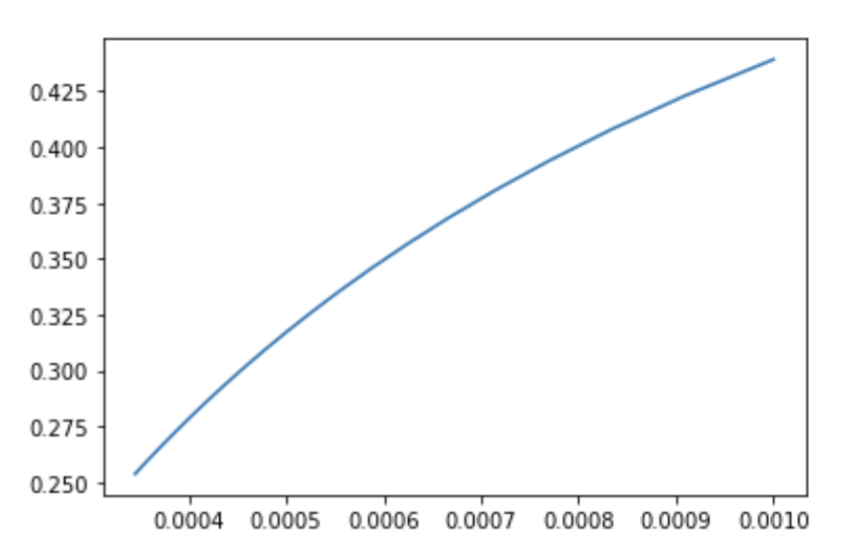
\includegraphics{1.png}
\end{center}

Построим график зависимости ошибки от шага по пространству 

\begin{center}
	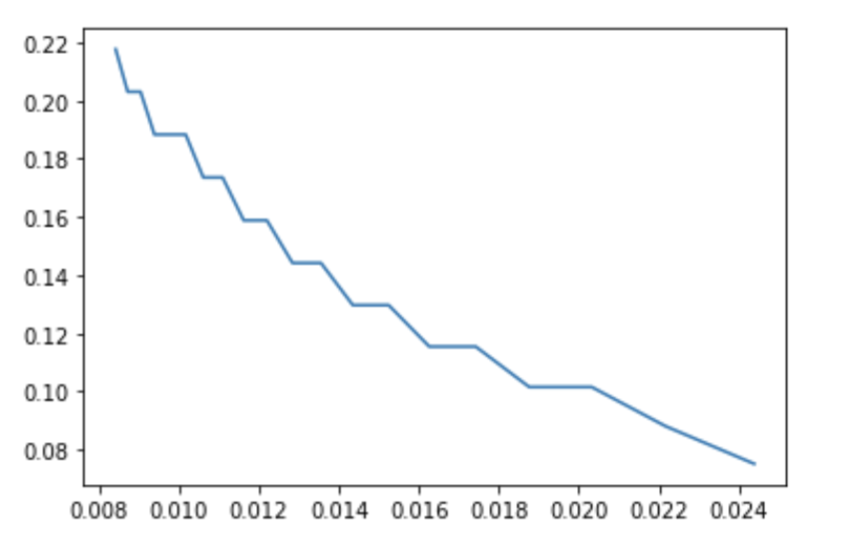
\includegraphics{2.png}
\end{center}

Как мы видим при меньших шагах получаем результы худшие результаты. Это связано с тем, что аппроксимация условная. 
Теперь посторим график с постоянной $\sigma$ 

\begin{center}
	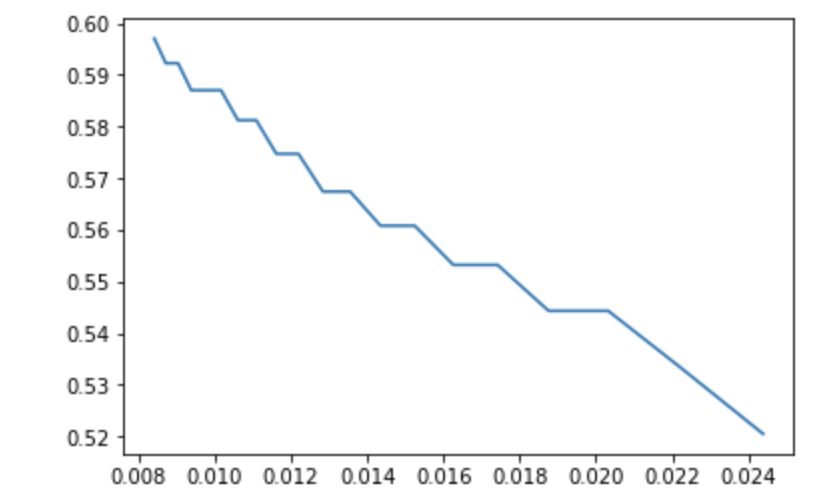
\includegraphics{3.png}
\end{center}

\section{Результаты расчётов}
Расчетаем несколько задач: 

1) $f = 0, \phi_{left} = 0, \phi{right} = 1, \phi{top} = \phi_{bottom} = x, u_0 = 0.5$

\begin{center}
	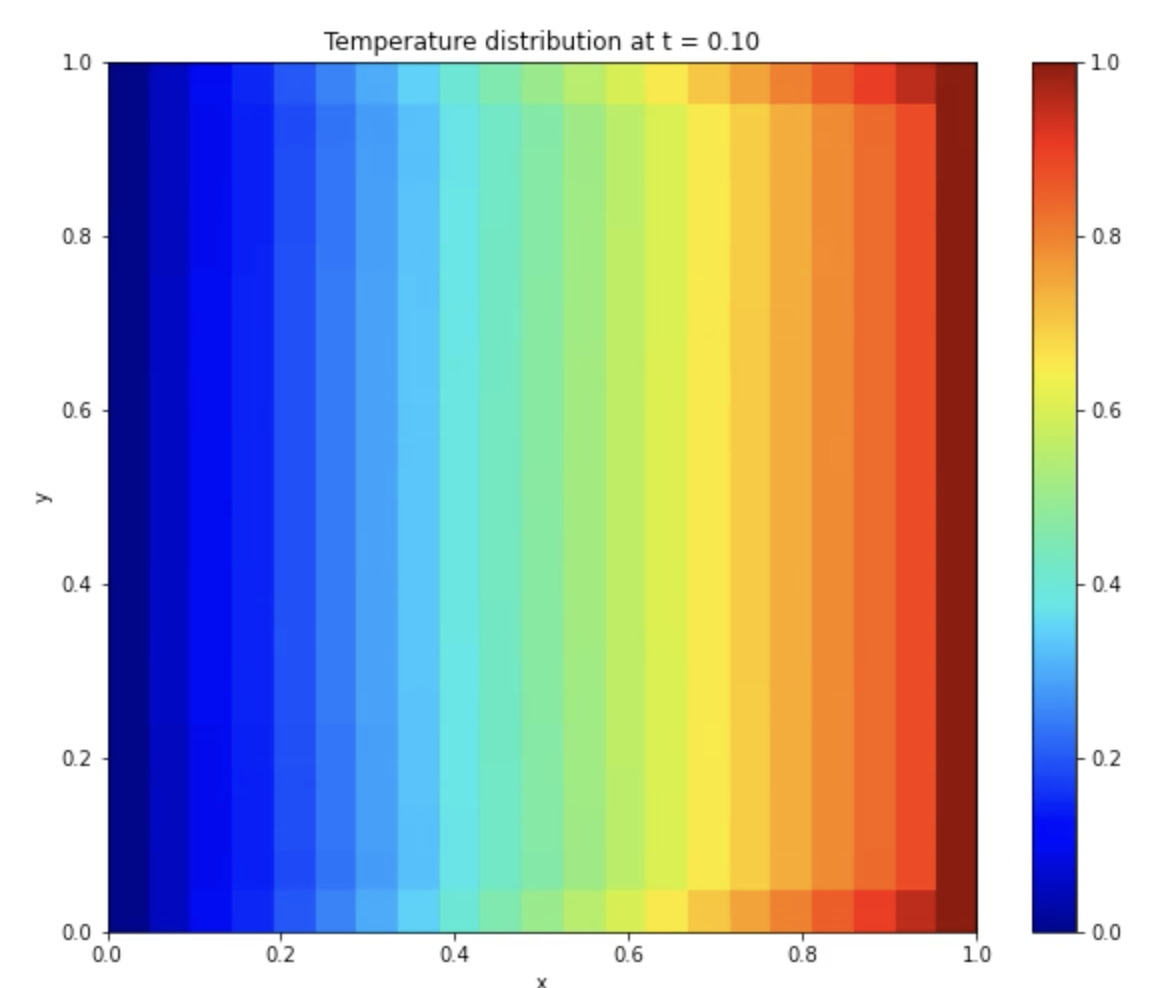
\includegraphics[width=500pt]{linear.png}
\end{center}



2) $f = 100 (0.4 < x < 0.6, 0.4 < y < 0.6), \phi_{left} = 0, \phi{right} = 0, \phi{top} = \phi_{bottom} = 0, u_0 = 0.5$

\begin{center}
	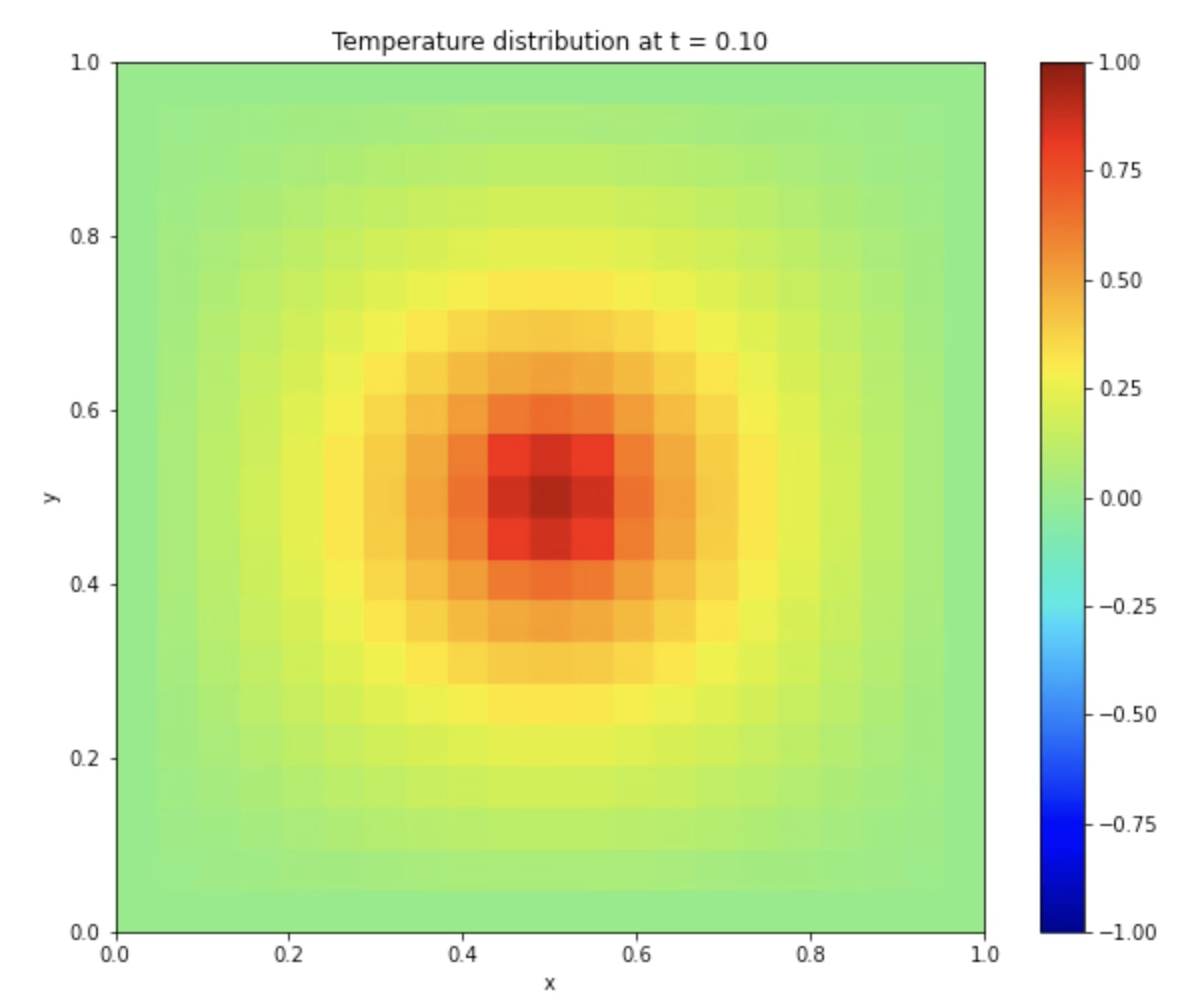
\includegraphics[width=500pt]{center.png}
\end{center}


2) $f = 1000 * sin(2 * \pi * t) (0.4 < x < 0.6, 0.4 < y < 0.6), \phi_{left} = 0, \phi{right} = 0, \phi{top} = \phi_{bottom} = 0, u_0 = \sin{(x + y)}$

\begin{center}
	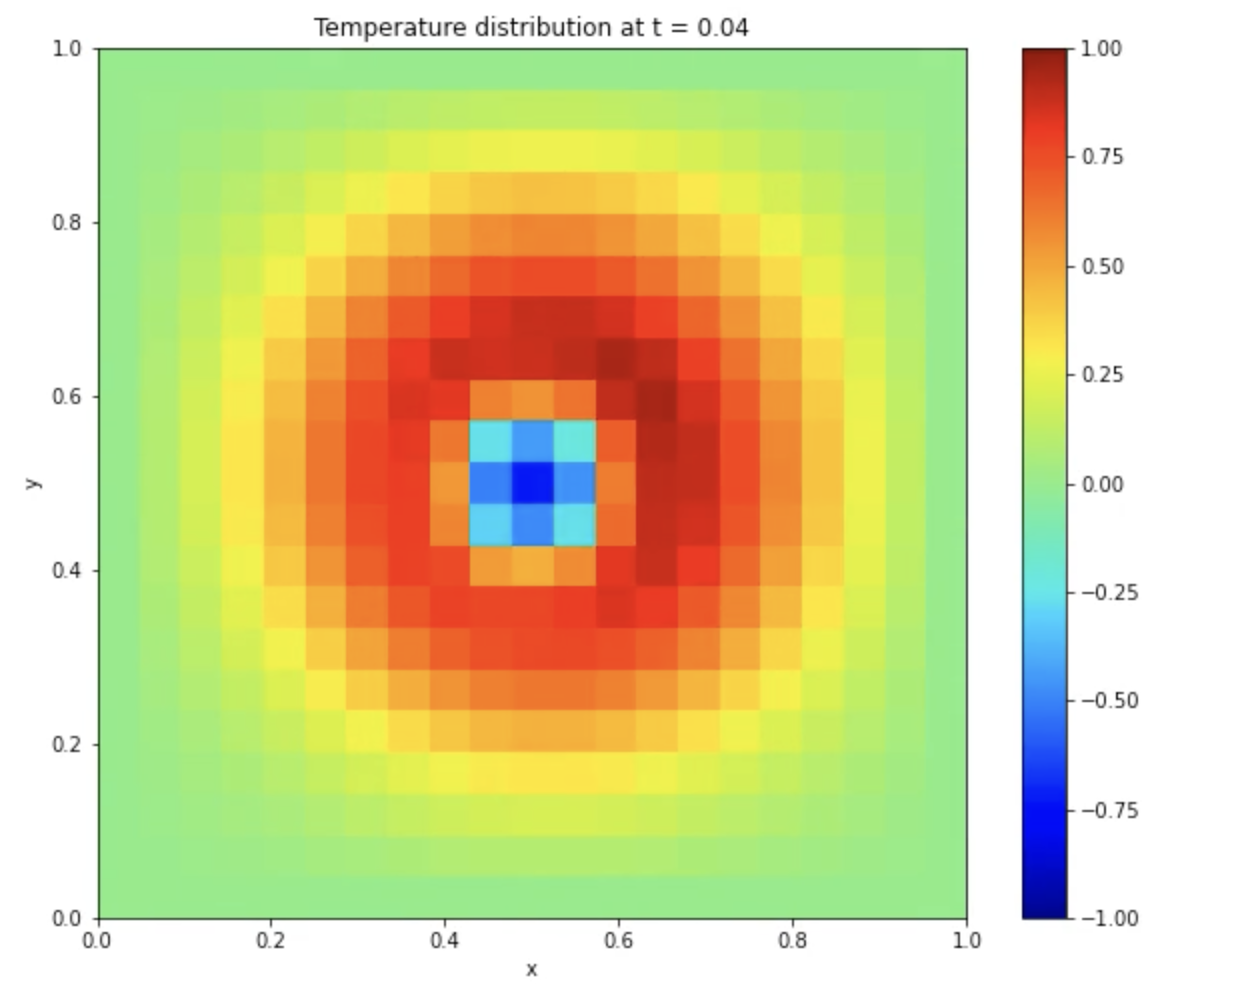
\includegraphics[width=500pt]{dymanic.png}
\end{center}

\section{Выводы}

Таким образом, выполненная курсовая работа позволила изучить метод расщепления для численного решения уравнения теплопроводности, провести тестирование программы на различных задачах и сделать выводы о его эффективности.

1. Математическая постановка задачи о распределении температуры в металлической пластине, получающей тепло от источника тепла.

2. В задаче численного решения принят метод расщепления, позволяющий эффективно решать уравнение теплопроводности в двумерном пространстве.

3. Изучены свойства, аппроксимация и устойчивость метода. Доказано, что метод абсолютно устойчив и имеет аппроксимацию второго порядка по пространству и первого порядка по времени.

4. Программа была протестирована на точном решении, что позволило оценить ее практическую точность и сходимость отдельных шагов во времени и пространстве.

5. Проведены расчеты для различных задач с заданными параметрами и начальными условиями, в результате чего получено графическое представление распределения температуры внутри пластины.

6. Результаты расчетов и испытаний позволяют сделать выводы о пригодности метода расщепления для решения задач распределения температуры.



\section{Список литературы}

\url{https://intuit.ru/studies/courses/1170/213/lecture/5503?page=2}

\end{document}